\section{Suivi des objets}
Nous avons vu précédemment qu’étant donné que les blobs sont détectés de la gauche vers la
droite et de haut en bas, lorsqu’on effectue une rotation de deux doigts, la détection des blobs
s’inverse quand le doigt en dessous de l’autre passe au-dessus. Or, pour n’importe quelle application
utilisant une interface tactile, il est indispensable de détecter et de suivre un doigt donné sans qu’il
soit inversé ou confondu avec un autre. En somme, nous avons répondu à la question « comment
détecter un input de type touch ? », mais pas à la question « comment effectuer le suivi de ces
input ?».

\subsection{Calcul des distances généralisées}
La méthode employée pour effectuer un tel suivi consiste à comparer les blobs de deux images
consécutives. De cette comparaison va résulter une matrice dont les lignes (resp. les colonnes)
correspondent aux blobs détectés de la première image (resp. de l’image suivante). Les valeurs
contenues dans cette matrice sont les distances relatives entre chaque blob de la première image et
chaque blob de l’image suivante. Ensuite, en traitant ces informations d’une manière que nous
verrons plus tard, il est possible d’attribuer à un ancien blob un des nouveaux blobs qui lui
correspond le mieux, mais de détecter aussi l’apparition ou la disparition d’un blob.\\

Pour le calcul des distances, il vient naturellement à l’esprit d’utiliser une distance euclidienne.
En effet, entre deux images, un doigt ne peut bouger que très peu et donc les blobs qui lui
correspondent sur les deux images sont probablement très proches (à condition bien sûr d’avoir une
cadence d’acquisition raisonnablement élevée). De plus, si un des nouveaux blobs se trouve loin de
tous les anciens blobs, on peut en déduire qu’il s’agit d’une apparition d’un blob. Inversement, si un
ancien blob se trouve loin de tous les nouveaux, il correspond probablement à un doigt qui n’est plus
en contact avec la surface tactile. Cependant, il est possible d’améliorer encore le suivi des objets en
faisant intervenir d’autres paramètres dans cette distance ; on obtient alors une distance
généralisée. Comme autres paramètres, nous pouvons prendre par exemple la surface, l’orientation
ou encore la forme. En utilisant une telle distance plus précise, on obtient de ce fait un meilleur suivi
moins sujet aux confusions.\\

Cependant, dès lors que l’on fait intervenir plusieurs paramètres dans la distance, un problème
se pose : comment s’assurer de l’équivalence entre l’impact des variations de chaque paramètre ?
Prenons comme exemple une distance généralisée dans laquelle interviendraient la distance
euclidienne et la surface que l’on additionnerait sans coefficients :
\begin{framed}
$$(d(blob1, blob2) = (position blob1 - position blob2) 
				+ (surface blob1 - surface blob2 )$$
\end{framed}
La distance étant exprimée en mètre et la surface en mètre carré, les variations de ces deux paramètres
n’ont pas du tout le même poids. Une variation de surface (en termes d’unité) entraînerait une plus
grande variation de la distance généralisée qu’une variation de la distance euclidienne ; c’est pourquoi 
nous prenons la racine carrée de la surface plutôt que la surface elle-même. Par ce
procédé, les deux paramètres ont un impact uniforme sur la distance généralisée.\\

Revenons à notre matrice des distances généralisées dont les lignes représentent les blobs de
l’image précédente et les colonnes les blobs de l’image courante. Une fois construite, trois cas se
présentent :
\begin{itemize}
 \item il y a plus d’anciens blobs que de nouveaux : on cherche la distance minimum pour
chaque nouveau blob (pour chaque colonne). En procédant ainsi, des anciens blobs
(des lignes) ne seront déterminés proches d’aucun nouveau blob. On éliminera plus
tard ces blobs.\\

$\begin{pmatrix}
   2 & 9\\
   5 & 0.5\\
   7 & 1
\end{pmatrix}$\\

  \item Il y a plus de nouveaux blobs que d’anciens : inverse du premier cas\\
  
$\begin{pmatrix}
   2 & 9 & 3\\
   5 & 0.5 & 7\\
\end{pmatrix}$\\

  \item Il y a autant d’anciens que de nouveaux blobs : pour chaque ligne et pour chaque
colonne, un minimum sera trouvé. A priori, à chaque ancien blob sera assigné un nouveau.\\

$\begin{pmatrix}
   2 & 9 & 34\\
   57 & 124 & 29\\
   7 & 3 & 41
\end{pmatrix}$\\

\end{itemize}

Une fois que l’on a effectué ce premier traitement, on regarde les valeurs minimums
trouvées et on élimine les valeurs supérieures à un seuil que l’on aura préalablement déterminé. En
effet, si un couple ancien blob – nouveau blob a été trouvé, qui nous dit qu’il s’agit réellement du
même objet ? Si leur distance est supérieure à ce seuil, c’est que l’on est face probablement à la
disparition et à l’apparition simultanées de blobs qui n’ont rien à voir entre eux. La matrice
résultante contient donc les valeurs retenues et des valeurs sentinelles lorsqu’une valeur a été
écartée.\\

$\begin{pmatrix}
   2 & -1 & -1\\
   -1 & -1 & 29\\
   -1 & 3 & -1
\end{pmatrix}$
=>
$\begin{pmatrix}
   2 & -1 & -1\\
   -1 & -1 & -1\\
   -1 & 3 & -1
\end{pmatrix}$\\

\subsection{Etiquetage des blobs}
Arrivé à ce stade du traitement, il s’agit d’analyser les valeurs calculées et retenues pour
assigner les étiquettes des anciens blobs aux nouveaux blobs correspondants et de traiter la
disparition ou l’apparition éventuelles de blobs.\\

Que nous dit la matrice ? Si pour une ligne, aucune valeur n’a été retenue, c’est qu’aucun blob
de l’image courante n’a été trouvé pour correspondre au blob de l’image précédente de cette ligne ;
c’est donc qu’il a disparu. On supprime donc son étiquette. Ensuite, si pour une colonne, aucune
valeur n’a été retenue, c’est qu’aucun blob de l’image précédente n’a été trouvé pour correspondre
au blob de l’image courante de cette colonne ; c’est donc que ce blob vient d’apparaître. On lui
attribue donc une nouvelle étiquette. Enfin, pour les valeurs retenues, on récupère le couple ligne –
colonne et on attribue l’étiquette de l’ancien blob de cette ligne au nouveau blob de cette colonne.
On a réussi à effectuer un suivi des objets détectés.\\

\begin{figure}[H]
      \center
      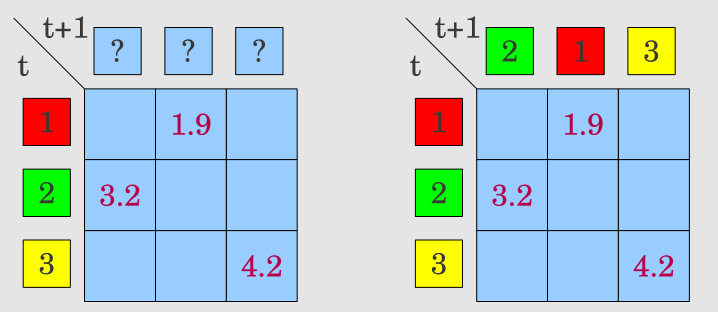
\includegraphics[width=12cm]{ressources/tp6/matrices.png}
      \caption{Attribution des étiquettes}
\end{figure}

Il va de soi qu’un tel système n’est pas infaillible. Des confusions sont encore possibles, mais
cela constitue une méthode très performante en matière de suivi d’objets. Il est possible, en ajoutant
d’autres paramètres, d’obtenir un système plus minutieux dans l’attribution d’étiquettes. Cependant,
il s’agit d’obtenir un compromis raisonnable entre robustesse et flexibilité.\\

\subsection{Envoi de messages par TUIO}
Un serveur TUIO fournit une interface permettant de gérer un suivi des doigts qui sont définis
en tant que curseurs. A chaque image, l’application soumet le résultat du traitement vu
précédemment au serveur qui se charge de garder en mémoire les curseurs avec des informations de
position ou encore de datation. Cette interface permet d’envoyer des messages relatifs à chaque
image qui informent de l’apparition, de la disparition et de la mise à jour de curseurs. Ce serveur
peut ainsi notifier un client des événements impliquant un changement dans les contacts entre les
objets et la surface tactile. L’application utilisant une interface multi-touch que nous allons
programmer pour la suite de ce cours sera ce client et utilisera les informations du serveur TUIO afin
de remplir les tâches qui lui incombent.
